% Chapter 7

\chapter{Background Processes} % Chapter title

\label{ch:background_processes} 

%----------------------------------------------------------------------------------------

This analysis is fundamentally a search for Supersymmetry in events with two leptons whose invariant mass is consistent with a Z boson. Additional event selections are made to reduce Standard Model processes relative to potential Supersymmetric processes, defined by simplified models discussed in \autoref{sec:simplified_models}. Supersymmetric events typically have large amounts of \MET, \HT (the scalar sum of the \pT of objects in the event), and many jets. All of these features can help isolate these events from backgrounds. To understand what cuts would optimize the sensitivity of the search, it is essential to first understand what these Standard Model backgrounds are. 

\begin{centering}
\begin{figure}[bth]
\myfloatalign
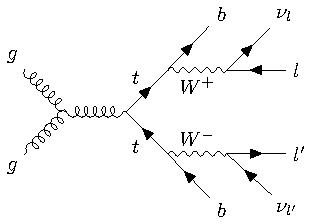
\includegraphics[width=.70\linewidth]{feynman/ttbar.pdf}
\caption{An example Feynman diagram of \ttbar production and decay.}
\label{fig:ttbar}
\end{figure}
\end{centering}

\paragraph{\ttbar} is the largest background for this search. \autoref{fig:ttbar} shows an example of this process, which can decay to many jets, leptons, and neutrinos, which are seen in the detector as \MET. Thus, \ttbar naturally has high \MET and \HT, jets, and leptons from two different W boson decays, which may coincidentally form an invariant mass on the Z peak. These events are very difficult to separate from potential signals, though keeping the mass window small and increasing \MET and \HT above the typical values for \ttbar events can help reduce them.

\begin{centering}
\begin{figure}[bth]
\myfloatalign
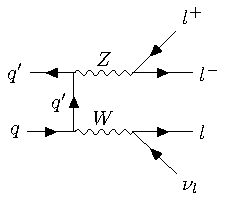
\includegraphics[width=.70\linewidth]{feynman/diboson.pdf}
\caption{An example Feynman diagram of the production and decay of a WZ event.}
\label{fig:diboson}
\end{figure}
\end{centering}

\paragraph{diboson} production is the next leading background. These events can contain real Z bosons and will peak on-Z like a signal. In addition, in events like \autoref{fig:diboson}, an additional W boson can decay to another lepton and a neutrino, providing \MET. The pictured process can occur with associated jets, but at reduced rates, so adding a jet requirement to the signal region can help reduce these events. If the W boson in this diagram instead decayed to two jets, there would be no true \MET from a neutrino, so a \MET cut in conjunction with a jet cut is very effective in reducing the total diboson background. 

\begin{centering}
\begin{figure}[bth]
\myfloatalign
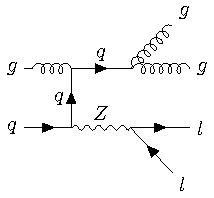
\includegraphics[width=.70\linewidth]{feynman/zjets.pdf}
\caption{An example Feynman diagram of the production and decay of a \dyjets event.}
\label{fig:zjets}
\end{figure}
\end{centering}

\paragraph{\dyjets} processes are very common but, as shown in \autoref{fig:zjets}, don't produce any true \MET or a very large number of jets. Thus a high \HT cut can help reduce this background, but a \MET cut is the most powerful. Events with very mismeasured jets or leptons can fake high \MET, but these drastic mismeasurements are rare. 

Other processes can contribute to the Standard Model background at lower rates. Processes similar to \dyjets but with a W boson instead of a Z have real \MET from leptonic W decays, but only one lepton. However, a fake or non-prompt lepton can cause these events to look very similar to simulated signals. Additionally, there are rare processes such as \ttbar in association with bosons that will also be difficult to separate from signal processes.

\section{Monte Carlo Samples} 

To precisely compare simulated signal to backgrounds, \ac{MC} samples are generated for each of these processes. \autoref{tab:MC} details the method used to produce each sample. With these and the simulated background, optimizations on a signal regioin can be made to maximize potential for discovery or exclusion of simplified Supersymmetric models. These comparisons and the signal region definition can be found in \autoref{sec:sr}.

\begin{sidewaystable*}[ht]
\begin{center}
\scriptsize
\begin{tabular}{l c c c c c }
\hline
Physics process &  Generator  & Parton & Cross section & Tune & PDF set\\
                &             & Shower &              &      & \\
%\hline\hline
\noalign{\smallskip}\hline\noalign{\smallskip}
$t\bar{t}+W$ and $t\bar{t}+Z$~\cite{ATL-PHYS-PUB-2016-005,Garzelli:2012bn}& {\sc MG5\_aMC@NLO}        & {\sc Pythia} 8.186 & NLO \cite{Campbell:2012,Lazopoulos:2008} & {\sc A14} & NNPDF23LO\\
$t\bar{t}+WW$~\cite{ATL-PHYS-PUB-2016-005}      & {\sc MG5\_aMC@NLO}          & {\sc Pythia} 8.186 & LO \cite{Alwall:2014hca} & {\sc A14}  &  NNPDF23LO\\
$t\bar{t}$~\cite{ATL-PHYS-PUB-2016-004}         & {\sc Powheg Box v2} r3026   & {\sc Pythia} 6.428 & NNLO+NNLL \cite{ttbarxsec1,ttbarxsec2}          &\sc{Perugia2012}     &NLO CT10\\
Single-top ($Wt$)~\cite{ATL-PHYS-PUB-2016-004}  & {\sc Powheg Box v2} r2856   & {\sc Pythia} 6.428 & Approx. NNLO \cite{Kidonakis:2010b}& \sc{Perugia2012}    &NLO CT10\\ 
$WW$,                      & \multirow{2}{*}{\sherpa\ 2.1.1} & \multirow{2}{*}{\sherpa\ 2.1.1} & \multirow{2}{*}{NNLO \cite{diboson1,diboson2}} & \multirow{2}{*}{\sherpa\ default} & \multirow{2}{*}{NLO CT10} \\
$WZ$ and $ZZ$~\cite{ATL-PHYS-PUB-2016-002} &&& \\ 
$Z/\gamma^{*}(\rightarrow \ell \ell)$ + jets~\cite{ATL-PHYS-PUB-2016-003}& \sherpa\ 2.1.1           & \sherpa\ 2.1.1  &NNLO \cite{DYNNLO1,DYNNLO2}       & \sherpa\ default     &NLO CT10\\
\noalign{\smallskip}\hline\noalign{\smallskip}
\end{tabular}
\caption{Simulated background event samples used in this analysis with the corresponding matrix element and parton shower generators, 
cross-section order in $\alpha_{\text{s}}$ used to normalise the event yield, underlying-event tune and PDF set. 
}
\label{tab:MC}
\end{center}
\end{sidewaystable*}